\documentclass[12pt]{article}
\usepackage{amsmath}
\usepackage{arydshln}
\usepackage{hhline}
\usepackage{amsmath}
\usepackage{graphicx}
\usepackage{float}
\usepackage{chngcntr}
\usepackage[T1]{fontenc}
\usepackage[utf8]{inputenc}
\usepackage{subcaption}
\DeclareMathOperator{\sign}{sgn}
\usepackage{comment}
\usepackage{breqn}
\usepackage{bm}
\usepackage{tabularx,ragged2e,booktabs,caption}
\newcolumntype{C}[1]{>{\Centering}m{#1}}
\renewcommand\tabularxcolumn[1]{C{#1}}
\usepackage{mathtools}
\renewcommand{\arraystretch}{1.5}
\title{Semitrailer modelling}
\author{MarsvinTech}

\begin{document}
\maketitle

\section{System description}
\begin{figure}[H]
    \centering
    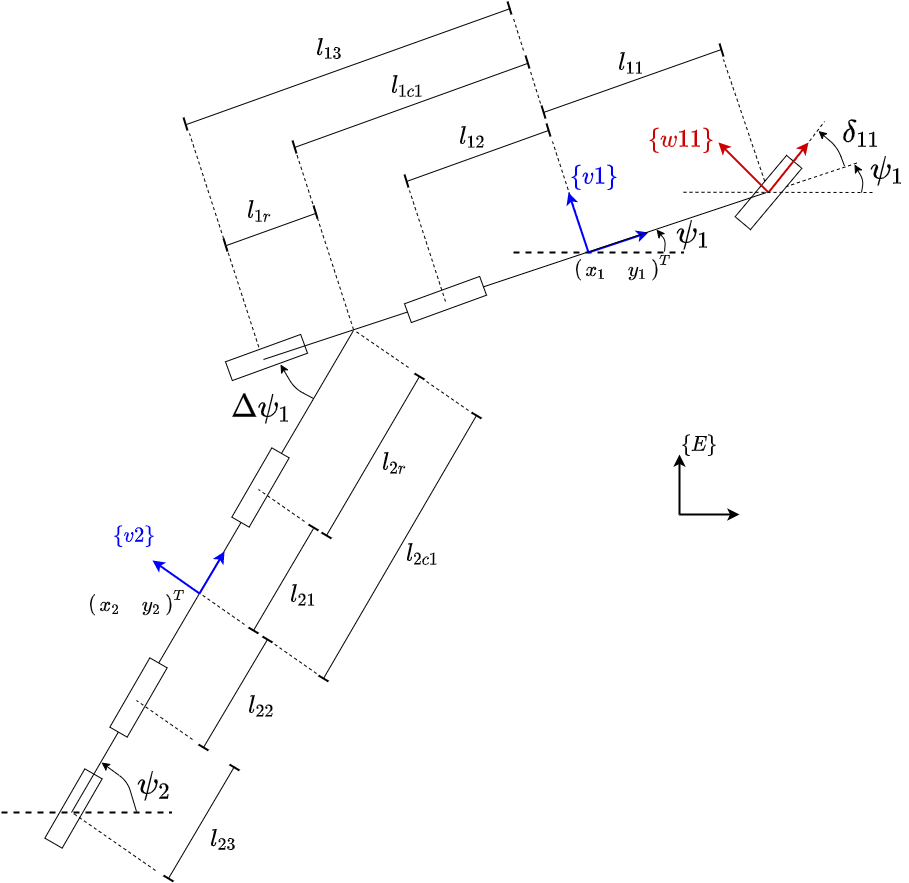
\includegraphics[scale=0.5]{images/semitrailer_modelling_1.png}
    \caption{Semitrailer model: Single axle bicycle model}
    \label{semitrailer_system}
\end{figure}

\begin{figure}[H]
    \centering
    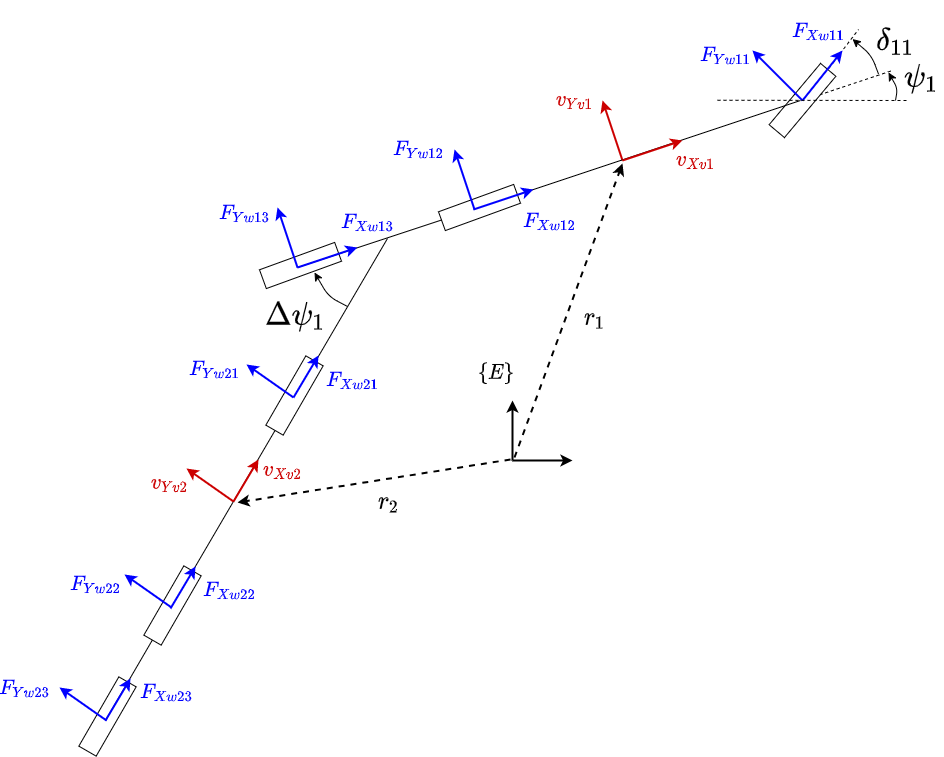
\includegraphics[scale=0.5]{images/semitrailer_modelling_forces.png}
    \caption{Semitrailer model: Position and forces vectors.}
    \label{semitrailer_system_forces}
\end{figure}
\begin{table}[H]
\begin{tabular}{p{4cm} p{10cm}}
$\mathcal{N}_u$&: Set of numbers of vehicle units.\\
$\mathcal{N}_a$&: Set of numbers of vehicle axles.\\
$j$ &: Vehicle unit number variable, where $j \in \mathcal{N}_u$.\\
$k$ &: Vehicle axle number variable, where $k \in \mathcal{N}_a$.\\
Frame $\{ E \}$& : Axis system fixed in the earth frame or reference frame.\\
Frame $\{ vj \}$& : Axis system fixed in the center of gravity (CoG) in vehicle unit $j$.\\
Frame $\{ wjk \}$& : Axis system fixed in unit $j$ axle $k$.\\
$R_z$ &: Rotation around $z$-axis.\\
$R_{vj}$ & : Rotation matrix of Frame $\{ vj \}$ with respect to Frame $\{ E \}$.\\
$R_{wjk}$ & : Rotation matrix of Frame $\{ wjk \}$ with respect to Frame $\{ E \}$.\\
$\psi_j$ &: Inclination angle of vehicle unit $j$ with respect to x-axis of Frame $\{ E \}$. Unit: $rad$.\\
$\Delta \psi _j$ &: Angle between vehicle unit $j$ and unit $j+1$. Unit: $rad$.\\
$\delta_{jk}$ &: Inclination angle of Frame $\{ wjk \}$ with respect to $x$-axis of Frame $\{ vj \}$. Unit: $rad$.\\
$r_j = \begin{pmatrix} x_j & y_j \end{pmatrix}^T$ & : Position vector of CoG of vehicle unit $j$ with respect to Frame $ \{ E \}$. Unit: $m$\\
$v_{j} = \dot{r_j} = \begin{pmatrix} \dot{x}_j & \dot{y}_j \end{pmatrix}^T$ & : Velocity vector of CoG of vehicle unit $j$ with respect to Frame $ \{ E \}$. Unit: $ \displaystyle \frac{m}{s}$\\
$v_j^{vj} = \begin{pmatrix} v_x & v_y \end{pmatrix}^T$ & : Velocity vector of CoG of vehicle unit $j$ with respect to Frame $ \{ vj \}$. Unit: $ \displaystyle \frac{m}{s}$\\
$a_j = \ddot{r}_j = \begin{pmatrix} \ddot{x}_j & \ddot{y}_j \end{pmatrix}^T$ & : Velocity vector of CoG of vehicle unit $j$ w.r.t Frame $ \{ E \}$. Unit: $ \displaystyle \frac{m}{s^2}$\\
$r_{jk}$ &: Position vector of CoG of vehicle axle $k$ unit $j$ with respect to Frame $\{ E\}$. Unit: $m$.\\
\end{tabular}
\end{table}

\begin{table}[H]
\begin{tabular}{p{4cm} p{10cm}}
$r_{jk}^{vj}$ &: Position vector of vehicle axle $k$ unit $j$ with respect to Frame $\{ vj\}$. Unit: $m$.\\
$v_{jk} = \dot{r}_{jk}$ &: Velocity vector of vehicle axle $k$ unit $j$ with respect to Frame $\{ E\}$. Unit: $ \displaystyle \frac{m}{s}$.\\
$v_{jk}^{vj} = \dot{r}_{jk}^{vj}$ &: Velocity vector of vehicle axle $k$ unit $j$ with respect to Frame $\{ vj\}$. Unit: $ \displaystyle \frac{m}{s}$.\\
$v_{jk}^{wjk} = \dot{r}_{jk}^{wjk}$ &: Velocity vector of vehicle axle $k$ unit $j$ with respect to Frame $\{ wjk\}$. Unit: $ \displaystyle \frac{m}{s}$. \\
$m_j$ &: Mass of vehicle unit $j$. Unit: $Kg$\\
$J_j$ &: Inertia around $z$-axis of vehicle unit $j$. Unit: $ kg.m^2$.\\
$l_{jk}$ &: Distance from CoG of vehicle unit $j$ to axle $k$. Unit: $m$.\\
$C_{yjk}$ &: Cornering stiffness of vehicle axle $k$ unit $j$. Unit: $ \displaystyle \frac{N}{rad}$.\\

\end{tabular}
\end{table}


\section{Rotation matrices}
\begin{equation}
    R_z (\theta) = \begin{pmatrix} \cos{\theta} & - \sin{\theta} \\ \sin{\theta} & \cos{\theta} \end{pmatrix}
\end{equation}
\begin{equation}
    R_{v1} = R_z (\psi_1)
\end{equation}
\begin{equation}
    R_{v2} = R_z (\psi_2)
\end{equation}
\begin{equation}
    R_{w11} = R_z (\delta_{11})
\end{equation}


Some properties for rotation matrices,
\begin{equation}
R^{-1} = R^T    
\end{equation}
\begin{equation}
R^{n}_{p} = R^{n}_m R^{m}_p     
\end{equation}
\begin{equation}
    r^n = R^n_p r^p
\end{equation}
where $r^n$ is the vector $r$ represented in the Frame ${n}$ and $R^n_p$ is the rotation matrix of Frame $\{ p \}$ with respect to Frame $\{ n \}$.
\section{Semitrailer dynamics using Euler-Lagrange equation}
Some manipulations were done using the Euler-Lagrange equation in order to obtain the state-space equation. This steps are a bit different than other steps published in some articles and books. These steps help to compute the differential equation use for the state-space expression.

The Euler-Lagrange equation is defined by,
\begin{equation}
    \frac{d}{dt} \Big( \frac{\partial \mathcal{L}(q,\dot{q})}{\partial \dot{q}} \Big) - \frac{\partial \mathcal{L}(q,\dot{q})}{\partial q} = Q
\end{equation}
where $q$ is the generalized coordinates, $\mathcal{L} (q,\dot{q})$ is the Lagrangian and $Q$ are the generalized forces of the system.

The Lagrangian is defined as,
\begin{equation}
\mathcal{L} (q,\dot{q}) = T(q,\dot{q}) - V(q)    
\end{equation}
where $T$ is the kinetic energy and $V$ is the potential energy. For car modeling, the potential energy can be neglected, therefore the Euler-Lagrange equation can be expressed as,

\begin{equation} \label{eq_el_1}
    \frac{d}{dt} \Big( \frac{\partial T(q,\dot{q}) }{\partial \dot{q}} \Big) - \frac{\partial T(q,\dot{q}) }{\partial q} = Q
\end{equation}

Then by using chain-rule, the following equivalent expressions can be obtained,

\begin{equation}
\label{eq_el_2}
  \frac{d}{dt} \Big( \frac{\partial T(q,\dot{q}) }{\partial \dot{q}} \Big) = \frac{\partial }{\partial q} \Big( \frac{\partial T(q,\dot{q})}{\partial \dot{q}} \Big) \dot{q} + \frac{\partial }{\partial \dot{q}} \Big( \frac{\partial T(q,\dot{q})}{\partial \dot{q}} \Big) \ddot{q}  
\end{equation}
using \eqref{eq_el_2} in \eqref{eq_el_1} and solving for $\ddot{q}$,
\begin{equation}
    \ddot{q} =  \Bigg(  \frac{\partial }{\partial \dot{q}} \Big( \frac{\partial T(q,\dot{q})}{\partial \dot{q}} \Big) \Bigg)^{-1} \Bigg( \frac{ \partial T(q,\dot{q})}{\partial q} - \frac{\partial }{\partial q} \Big( \frac{\partial T(q,\dot{q})}{\partial \dot{q}} \Big) \dot{q} + Q \Bigg)
\end{equation}
\subsection{Generalized coordinates}
\begin{equation} \label{Generalized_coordinates_eq}
    q = \begin{pmatrix} x_{1} \\ y_{1} \\ \psi_1 \\ \Delta \psi_1 \end{pmatrix} \quad \longrightarrow \quad \dot{q} = \begin{pmatrix} \dot{x}_{1} \\ \dot{y}_{1} \\ \dot{\psi} _1 \\ \Delta \dot{\psi}_1 \end{pmatrix} \quad \longrightarrow \quad \ddot{q} = \begin{pmatrix} \ddot{x}_{1} \\ \ddot{y}_{1} \\ \ddot{\psi} _1 \\ \Delta \ddot{\psi}_1 \end{pmatrix}
\end{equation}
\subsection{Kinetic energy}
The total kinetic energy for the semi-trailer combination is given by,
\begin{equation}
    T(q,\dot{q}) = \sum_{j \in \mathcal{N}_u} \Big( \frac{1}{2}m_j v_j^T v_j + \frac{1}{2}J_1\dot{\psi}_j^2 \Big) 
\end{equation}

\begin{equation}
    T(q,\dot{q}) = \frac{1}{2}m_1 v_1^T v_1 + \frac{1}{2}m_2 v_2^T v_2 + \frac{1}{2}J_1\dot{\psi}_1^2 + \frac{1}{2}J_2\dot{\psi}_2^2
\end{equation}
using chain rule, $\dot{r}$ can be calculated by,
\begin{equation}
    v_j = \dot{r}_j = \frac{\partial r _j}{\partial q}\dot{q}
\end{equation}
The following position vectors are defined,
\begin{equation}
    r_{1c1}^{vj} = \begin{pmatrix} - l_{1c1} \\ 0 \end{pmatrix} \quad , \quad r_{2c1}^{v2} = \begin{pmatrix} l_{2c1} \\ 0 \end{pmatrix}
\end{equation}
where $r_{jc1}^{v1}$ is the distance between center of gravity of vehicle unit $j$ and joint 1 represent in Frame $\{vj \}$.

Then, $r_2$ can be calculated as,
\begin{equation}
    r_2 = r_1 + R_{v1} r_{1c1}^{v1} - R_{v2} r_{2c1}^{v2} 
\end{equation}
Therefore, the position vectors of each center of gravity can be expressed as a function of $q$,
\begin{equation}
    r_1 (q) = \begin{pmatrix} x_1 \\ y_1 \end{pmatrix}
\end{equation}
\begin{equation}
    r_2 (q) = r_1 + R_{v1} \begin{pmatrix} - l_{1c1} \\ 0 \end{pmatrix} - R_{v2} \begin{pmatrix} l_{2c1} \\ 0 \end{pmatrix} 
\end{equation}
The translational velocities vector for center of gravity of vehicle unit $j$ can be calculated as, 
\begin{equation}
    v_j (q,\dot{q}) = \dot{r}_j = \frac{\partial r_j}{\partial q}\dot{q} \quad , \quad j \in \mathcal{N}_u
\end{equation}

Furthermore, you can calculate $\psi_2$ by,
\begin{equation}
    \psi _2 (q)= \psi _1 - \Delta \psi_1
\end{equation}

\subsection{Generalized forces}
The generalized forces can be calculated by,

\begin{equation}\label{Generalized_forces_general_eq}
    Q = \sum_{j \in \mathcal{N}_u} \sum_{k \in \mathcal{N}_a} \Big( \frac{\partial r_{jk}}{\partial q} \Big)^T F_{jk} + \sum_{j \in \mathcal{N}_u} \Big( \frac{\partial r_{j}}{\partial q} \Big)^T F_j 
\end{equation}

\begin{equation}
    \begin{split}
        Q = & \Big( \frac{\partial r_{11}}{\partial q} \Big)^T F_{11} + \Big( \frac{\partial r_{12}}{\partial q} \Big)^T F_{12} + \Big( \frac{\partial r_{13}}{\partial q} \Big)^T F_{13} + \quad \\ & \Big( \frac{\partial r_{21}}{\partial q} \Big)^T F_{21} + \Big( \frac{\partial r_{22}}{\partial q} \Big)^T F_{22} + \Big( \frac{\partial r_{23}}{\partial q} \Big)^T F_{23} + \quad \\
        & \Big( \frac{\partial r_{1}}{\partial q} \Big)^T F_{1} + \Big( \frac{\partial r_{2}}{\partial q} \Big)^T F_{2} 
    \end{split}
\end{equation}
where,
\begin{equation}\label{tyre_vector_position_fixed_frame}
    \begin{split}
        r_{11}^{v1} = \begin{pmatrix} l_{11} \\ 0 \end{pmatrix} \quad &, \quad r_{21}^{v2} = \begin{pmatrix} l_{21} \\ 0 \end{pmatrix} \\
        r_{12}^{v1} = \begin{pmatrix} - l_{12} \\ 0 \end{pmatrix} \quad &, \quad r_{22}^{v2} = \begin{pmatrix} - l_{22} \\ 0 \end{pmatrix} \\
        r_{13}^{v1} = \begin{pmatrix} - l_{13} \\ 0 \end{pmatrix} \quad &, \quad r_{23}^{v2} = \begin{pmatrix} -l_{23} \\ 0 \end{pmatrix}
    \end{split}
\end{equation}

In order to calculate $r_{jk}$, we can use homogeneous transformation matrices,

\begin{equation}
    \begin{pmatrix} r_{jk} \\ 1 \end{pmatrix} = H_{j} \begin{pmatrix} r_{jk}^{vj} \\ 1 \end{pmatrix} = \begin{pmatrix} R_{vj}  & r_j \\ \mathrm{0}_{1 \times 3} & 1 \end{pmatrix} \begin{pmatrix} r_{jk}^{vj} \\ 1 \end{pmatrix}
\end{equation}
where $H_j$ is the homogeneous transformation matrix of Frame $\{ vj \}$ with respect to Frame $\{ E \}$.  Then, the axles position vectors are calculated using,
\begin{equation}\label{Axles_position_eq}
    r_{jk} = r_j + R_{vj} r_{jk}^{vj} \quad , \quad (j,k) \in \mathcal{N}_u \times \mathcal{N}_a 
\end{equation}

The translational velocity vector of vehicle unit $j$ axle $k$ with respect to the earth frame ($v_{jk}$) can be define as,
\begin{equation}
    v_{jk} = \frac{\partial r_{jk}}{\partial q} \dot{q}
\end{equation}

This vector expressed in a wheel fixed frame can be calculated as,

\begin{equation}
    \begin{pmatrix} v_{Xwjk} \\ v_{Ywjk} \end{pmatrix} = \begin{cases} R_{wjk} v_{jk} \quad &, \quad (j,k) \in \{ (1,1) \} \\ R_{vj} v_{jk} \quad &, \quad (j,k) \in \mathcal{N}_u \times \mathcal{N}_a - \{ (1,1) \} \end{cases}
\end{equation}

Fig. \ref{semitrailer_system_forces} shows the forces acting on the semi-trailer combination. These forces are expressed in the fixed body frame of each unit and wheel. The forces acting on each center of mass are defined by,

\begin{equation}
    %\begin{split}
        F_{Xvj} = \begin{cases} F_{air} + F_{grav,j} \qquad& j=1 \\ F_{grav,j} \qquad& j=2 \end{cases} \\
    %\end{split}
\end{equation}
\begin{equation}
    F_{Yvj} = 0
\end{equation}

Assuming no longitudinal slip, small lateral slip and constant normal load, the lateral tyre forces can be approximated using, 

\begin{equation}\label{Lateral_Force_Results}
    F_{Ywjk} = - C_{Yjk} \frac{v_{Ywjk}}{v_{Xwjk}}
\end{equation}
where $C_{Yjk}$ is the tyre cornering stiffness of unit $j$ axle $k$.

The longitudinal tyre forces are generated by braking and propulsion and can be calculated as,

\begin{equation}\label{Forces_long_eq}
    F_{Xwjk} = \begin{cases} 
        F_{prop,jk} + F_{brake,jk} \quad &, \quad (j,k) \in \{  (1,2) \} \\
        0 \quad &, \quad \mathcal{N}_u \times \mathcal{N}_a - \{  (1,2) \}
    \end{cases}
\end{equation}

In order to calculate $F_j$ and $F_{jk}$, which are expressed with respect to Frame $\{ E \}$, the force vectors $(F_{xvj},F_{yvj})$ and $(F_{Xwjk},F_{Ywjk})$ should be rotated,

\begin{equation}
    F_j = R_{vj}\begin{pmatrix} F_{Xvj} \\ F_{Yvj} \end{pmatrix} \quad , \quad j \in \mathcal{N}_u
\end{equation}

\begin{equation}
    F_{jk} = \begin{cases}
         R_{wjk} \begin{pmatrix} F_{Xwjk} \\ F_{Ywjk} \end{pmatrix} \quad &, \quad (j,k) \in \{ (1,1) \} \\
        R_{vj} \begin{pmatrix} F_{Xwjk} \\ F_{Ywjk} \end{pmatrix} \quad &, \quad (j,k) \in \mathcal{N}_u \times \mathcal{N}_a - \{ (1,1) \}
    \end{cases}
\end{equation}

In this study the aerodynamic drag and gravitational forces are neglected. Therefore,
\begin{equation}
    F_{Xvj} = F_{Yvj} = 0 \quad , \quad j \in \mathcal{N}_u
\end{equation}


After all the operations, $\ddot{q}$ is estimated as a function of $\dot{x}_1$, $\dot{y}_1$, $\psi_1$, $\dot{\psi}_1$, $\Delta \psi _1$ and $\Delta \dot{\psi}_1$,

\begin{equation}
    \ddot{q} = \begin{pmatrix} \ddot{x}_1 \\ \ddot{y}_1 \\ \ddot{\psi}_1 \\ \Delta \ddot{\psi}_1 \end{pmatrix} = \mathcal{F} (\dot{x}_1,\dot{y}_1,\psi_1,,\dot{\psi}_1,\Delta \psi_1, \Delta \dot{\psi}_1)
\end{equation}

Since the velocity sensors on the car measure the longitudinal and lateral velocity of the car with respect of Frame $\{ v1 \}$. So we want something like,

\begin{equation}
    \ddot{q}_v = \begin{pmatrix} \dot{v}_{Xv1} \\ \dot{v}_{Yv1} \\ \ddot{\psi}_1 \\ \Delta \ddot{\psi}_1 \end{pmatrix} = \mathcal{F}(v_{Xv1},v_{Yv1},\psi_1,,\dot{\psi}_1,\Delta \psi_1, \Delta \dot{\psi}_1)
\end{equation}

In order to expressed the dynamics as a function of $v_{Xv1}$ and $v_{Yv1}$ instead of $\dot{x}_1$ and $\dot{y}_1$, the following rotation is done,

\begin{equation} \label{Rot_velocities_eq}
    \begin{pmatrix} \dot{x}_1 \\ \dot{y}_1 \end{pmatrix} = R_{v1} \begin{pmatrix} v_{Xv1} \\ v_{Yv1} \end{pmatrix}
\end{equation}
Moreover, calculating the derivative with respect to time,
\begin{equation}\label{Rot_eq_derivative}
    \begin{pmatrix} \ddot{x}_1 \\ \ddot{y}_1 \end{pmatrix} = \dot{R}_{v1} \begin{pmatrix} v_{Xv1} \\ v_{Yv1} \end{pmatrix} + R_{v1} \begin{pmatrix} \dot{v}_{Xv1} \\ \dot{v}_{Yv1} \end{pmatrix}
\end{equation}
Rewriting \eqref{Rot_eq_derivative},
\begin{equation}\label{velocity_fixed_unit_1_eq}
    \begin{pmatrix} \dot{v}_{Xv1} \\ \dot{v}_{Yv1} \end{pmatrix} = R_{v1}^T \begin{pmatrix} \ddot{x}_1 \\ \ddot{y}_1 \end{pmatrix} - R_{v1}^T \dot{R}_{v1} \begin{pmatrix} v_{Xv1} \\ v_{Yv1} \end{pmatrix} 
\end{equation}
\section{State-space model}

\subsection{Nonlinear state-space model: Lateral and longitudinal dynamics}
The following state and input vectors are selected for the semi-trailer nonlinear model,
\begin{equation}\label{NL_states_input}
    \mathcal{X}_{NL} = \begin{pmatrix} v_{Xv1} \\ v_{Yv1} \\ \Dot{\psi}_1 \\ \Delta \dot{\psi}_1 \\ \psi_1 \\ \Delta \psi_1 \end{pmatrix} \quad , \quad U_{NL} = \begin{pmatrix} \delta_{11} \\ F_{Xw12} \end{pmatrix}
\end{equation}
The nonlinear state-space model is defined by,
\begin{equation} \label{Nonlinear_state_space_eq}
    \Dot{\mathcal{X}}_{NL} = \begin{pmatrix} \Dot{v}_{Xv1}  \\ \Dot{v}_{Yv1} \\ \Ddot{\psi}_1 \\ \Delta \Ddot{\psi}_1 \\ \Dot{\psi_1} \\ \Delta \Dot{\psi_1} \end{pmatrix} = f_{NL}(\mathcal{X}_{NL},U_{NL})
\end{equation}
\subsection{Nonlinear state-space model: Only lateral dynamics}
In order to consider only lateral dynamics, it is possible to assume constant longitudinal velocity,
\begin{equation}
    v_{Xv1} = \mathrm{Constant}
\end{equation}
For constant longitudinal velocity, it is assumed that the sum of the projections to $x$-axis of Frame $\{ v1 \}$ of all the forces apply to the car is zero, i.e.,
\begin{equation}
    F_{Xw11} \cos{\delta_{11}} - F_{Yw11} \sin{\delta_{11}} + F_{Xw12} + F_{13} = 0
\end{equation}
The following state and input vectors are selected for the semi-trailer nonlinear model,
\begin{equation}\label{NL_states_input_vx}
    \mathcal{X}_{nl} = \begin{pmatrix} v_{Yv1} \\ \Dot{\psi}_1 \\ \Delta \Dot{\psi}_1 \\ \psi_1 \\ \Delta \psi_1 \end{pmatrix} \quad , \quad U_{nl} = \delta_{11}
\end{equation}
The nonlinear state-space model is defined by,
\begin{equation} \label{Nonlinear_state_space_vx_eq}
    \Dot{\mathcal{X}}_{nl} = \begin{pmatrix} \Dot{v}_{Yv1} \\ \Ddot{\psi}_1 \\ \Delta \Ddot{\psi}_1 \\ \Dot{\psi_1} \\ \Delta \Dot{\psi_1} \end{pmatrix} = f_{nl}(\mathcal{X}_{nl},U_{nl})
\end{equation}

\subsection{Linear state-space model: Lateral and longitudinal dynamics}
In order to linearize $f_{NL}$ (showed in \eqref{Nonlinear_state_space_eq}), the following equilibrium $ \begin{pmatrix} \mathcal{X}_e & \mathcal{Y}_e\end{pmatrix}^T$ point is selected,

\begin{equation}
    \mathcal{X}_e = \begin{pmatrix} v_{Xv1e} \\ v_{Yv1e} \\ \Dot{\psi}_{1e} \\ \Delta \Dot{\psi}_{1e} \\ \psi_{1e} \\ \Delta \psi_{1e} \end{pmatrix} = \begin{pmatrix} v_{Xv1d} \\ 0 \\ 0 \\ 0 \\ 0 \\ 0 \end{pmatrix} \quad , \quad U_e = \begin{pmatrix} \delta_{11e} \\ F_{Xw12e} \end{pmatrix} = \begin{pmatrix} 0 \\ 0 \end{pmatrix}
\end{equation}

where $v_{Xv1d}$ is the desired longitudinal velocity of the car. Additionally, around the equilibrium point no acceleration or braking is needed in order to keep constant longitudinal velocity. Therefore, $F_{Xw12e}$ can be approximated to zero,

\begin{equation}
    F_{Xw12e} = 0
\end{equation}

Then, $f_{NL}$ can be linearized around the equilibrium point ($\mathcal{X}_e$,$U_e$),

\begin{equation} \label{linear_expression_state}
    \dot{\mathcal{X}} = f_{LINEAR} = A (v_{Xv1d}) \mathcal{X} + B (v_{Xv1d}) U
\end{equation}

\subsection{Linear state-space model: Only lateral dynamics}
In order to linearize $f_{nl}$ (showed in \eqref{Nonlinear_state_space_vx_eq}), the following equilibrium $ \begin{pmatrix} \mathcal{X}_e & \mathcal{Y}_e\end{pmatrix}^T$ point is selected,

\begin{equation}
    \mathcal{X}_e = \begin{pmatrix} v_{Yv1e} \\ \Dot{\psi}_{1e} \\ \Delta \Dot{\psi}_{1e} \\ \psi_{1e} \\ \Delta \psi_{1e} \end{pmatrix} = \begin{pmatrix} 0 \\ 0 \\ 0 \\ 0 \\ 0  \end{pmatrix} \quad , \quad U_e =  \delta_{e} =  0 
\end{equation}

Then, $f_{nl}$ can be linearized around the equilibrium point ($\mathcal{X}_e$,$U_e$),

\begin{equation} \label{linear_expression_state}
    \dot{\mathcal{X}} = f_{linear} A (v_{Xv1d}) \mathcal{X} + B (v_{Xv1d}) U
\end{equation}

\end{document}
